\documentclass[landscape,footrule]{foils}
\usepackage[lecture-serie]{foiltex-extra}
\usepackage{crysymb}
\usepackage{graphics}
\usepackage[pdftex]{graphicx} 




\newcommand{\lecture}{Expectation-Maximisation algorithm \vspace*{0ex}\\for sequential models}
\newcommand{\lserie}{MTAT.03.227 Machine Learning}
\newcommand{\ldate}{May 22, 2019}
\newcommand{\lauthor}{Sven Laur}
\newcommand{\linst}{University of Tartu}
\graphicspath{{./illustrations/}}
\MyLogo{\lserie,\ EM for sequential models, \ldate}

\renewcommand{\VAR}{\mathbf{Var}}
\DeclareMathOperator{\diag}{diag}

\newcommand{\leqm}{\ \leq_m}

\newcommand{\pd}[1]{p\left[#1\right]}

\newcommand{\bigvskip}{\vskip 2em}
\newcommand{\lastline}{\vspace*{-2ex}}
\newcommand{\spreadappart}{\vspace*{\fill}}


\begin{document}
\titlefoil

\foilhead[-1cm]{Discrete time systems}

\centerline{
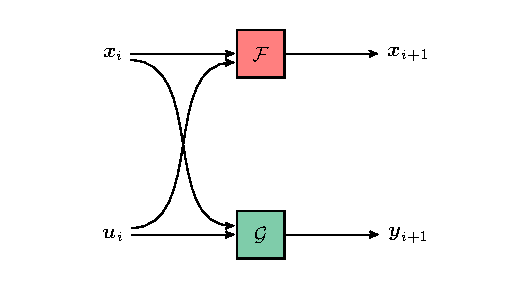
\includegraphics[scale=1.2]{nonlinear-control}
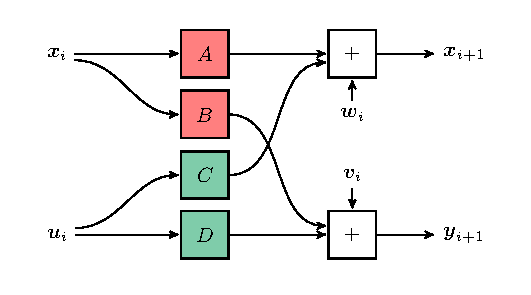
\includegraphics[scale=1.2]{linear-control}\hspace*{1cm}
}

Sequential models describe evolution of discrete time systems.
\begin{triangles}
\item System has an hidden state $\vec{x}_i$ evolving over state space $\XXX$.
\item We can make observations of the system $\vec{y}_i$ by measuring it.
\item We can influence the system by changing the control signal $\vec{u}_i$.
\item For linear system, uncontrollable noise $\vec{w}_i$ perturbs the state $\vec{x}_{i+1}$.  
\item For linear system, uncontrollable noise $\vec{v}_i$ perturbs the observation $\vec{y}_{i}$.  

\end{triangles}



\middlefoil{Enforcing temporal consistency}

\foilhead[-1cm]{Multinomial mixture model}

\illustration[scale=1.0]{multinomial-mixture-model}

Multinomial mixture model is a discrete time-system.
\begin{triangles}
\item The state space $\XXX$ is finite.
\item All states $x_1,\ldots,x_n$ are independently and identically distributed.
\item Mixture proportions $(\lambda_{x})_{x\in\XXX}$ quantify the corresponding probabilities.
\item Emission matrix $(\delta_{xy})_{x\in\XXX, y\in\YYY}$ the conditional probability of outcomes.  
\end{triangles}
\begin{align*}
\lambda_x&=\pr{x_i=x}\\
\delta_{xy}&=\pr{y_i=y|x_i=x}
\end{align*}

\foilhead[-1cm]{Discrete Hidden Markov Model}

\illustration[scale=1.0]{discrete-hidden-markov-model}

Discrete HMM is a refinement of multinomial mixture model.
\begin{triangles}
\item State transition probabilities $(\alpha_{x,x'})_{x,x'\in\XXX}$ are non-trivial.
\item Initial state probabilities $(\beta_{x})_{x\in\XXX}$ become important now.
\item Marginal state probabilities $(\lambda_{xi})_{x\in\XXX,i\in\NN}$ change over time.
\end{triangles}
\begin{align*}
\beta_x&=\pr{x_1=x}\\
\alpha_{xx'}&=\pr{x_{i+1}=x'|x_{i}=x}\\
\delta_{xy}&=\pr{y_i=y|x_i=x}
\end{align*}

\foilhead[-1cm]{Gaussian mixture model}

\illustration[scale=1.0]{gaussian-mixture-model}

Gaussian mixture model is a discrete time-system.
\begin{triangles}
\item The state space $\XXX$ is finite.
\item All states $x_1,\ldots,x_n$ are independently and identically distributed.
\item Mixture proportions $(\lambda_{x})_{x\in\XXX}$ quantify the corresponding probabilities.
\item Observations $\vec{y}_i$ are  determined by multivariate normal distributions.
\end{triangles}
\begin{align*}
\lambda_x&=\pr{x_i=x}\\
\vec{y}_i&\sim\NNN(\vec{\mu}_{x_i},\vec{\Sigma}_{x_i})
\end{align*}


\foilhead[-1cm]{Continuous Hidden Markov Model}

\illustration[scale=1.0]{continuous-hidden-markov-model}

Continuous HMM is a refinement of Gaussian mixture model.
\begin{triangles}
\item State transition probabilities $(\alpha_{x,x'})_{x,x'\in\XXX}$ are non-trivial.
\item Initial state probabilities $(\beta_{x})_{x\in\XXX}$ become important now.
\item Marginal state probabilities $(\lambda_{xi})_{x\in\XXX,i\in\NN}$ change over time.
\end{triangles}
\begin{align*}
\beta_x&=\pr{x_1=x}\\
\alpha_{xx'}&=\pr{x_{i+1}=x'|x_{i}=x}\\
\vec{y}_i&\sim\NNN(\vec{\mu}_{x_i},\vec{\Sigma}_{x_i})
\end{align*}



\foilhead[-1cm]{Multivariate linear transformations}

\illustration[scale=1.0]{multivariate-linear-transformation}

Multivariate linear transformation is a discrete time-system.
\begin{triangles}
\item The merged input and state space $\RR^{d}\times\RR^k$ is infinite. 
\item All states $\vec{x}_1,\ldots,\vec{x}_n$ are independently and identically distributed.  
\item States and observations disturbed by white gaussian noise.
\item Observations $\vec{y}_i$ are linear in inputs $\vec{u}_i$ and states $\vec{x}_i$.
\end{triangles}
\begin{align*}
\vec{x}_{i+1}&=\vec{0}\vec{x}_{i}+\vec{0}\vec{u}_{i}+\vec{w}_{i}, &\vec{w}_{i}&\sim \NNN(\vec{0}, \vec{I})\\
\vec{y}_i&=C\vec{x}_i+D\vec{u}_i+\vec{v}_i, &\vec{v}_{i}&\sim \NNN(\vec{0}, \vec{I})
\end{align*}



\foilhead[-1cm]{Kalman filter}

\illustration[scale=1.0]{kalman-filter}

Kalman filter is a refinement of multivariate linear transformation.
\begin{triangles}
\item Linear state evolution equation is non-trivial.
\item The initial state $\vec{x}_0$ is assumed to be fixed value.
\item States and observations disturbed by colored gaussian noise. 
\end{triangles}
\begin{align*}
\vec{x}_{i+1}&=A\vec{x}_{i}+B\vec{u}_{i}+\vec{w}_{i}, &\vec{w}_{i}&\sim \NNN(\vec{0}, \Sigma_1)\\
\vec{y}_i&=C\vec{x}_i+D\vec{u}_i+\vec{v}_i, &\vec{v}_{i}&\sim \NNN(\vec{0}, \Sigma_2)
\end{align*}


\middlefoil{EM-algorithm for HMM} 

\foilhead[-1cm]{Lower bound function}

The lower bound function used in the EM algorithm is current notation
\begin{align*}
F(\vec{q},\vec{\Theta})= -\sum_{\vec{x}}q(\vec{x})\cdot\log q(\vec{x})+
 \sum_{\vec{x}}q(\vec{x})\cdot\log\left(\pd{\vec{\Theta},\vec{x}|\vec{y}}\right)
\end{align*}

If we assign non-informative prior to the model parameters then in M-step it is sufficient to maximise the function

\begin{align*}
F_*=\sum_{\vec{x}}q(\vec{x})\cdot\log\left(\pd{\vec{y},\vec{x}|\vec{\Theta}}\right)
\end{align*}  

\foilhead[-1cm]{Probability assignment in E-step}

According to the theory the optimal probability assignment is
\begin{align*}
q(\vec{x})=\pr{\vec{x}|\vec{y},\vec{\Theta}_*}=\frac{\pd{\vec{y},\vec{x}|\vec{\Theta}_*}}{\pd{\vec{y}|\vec{\Theta}_*}}
\end{align*}
and thus we get
\begin{align*}
F_*=\frac{1}{\pd{\vec{y}|\vec{\Theta}_*}}\cdot\sum_{\vec{x}}\pd{\vec{y},\vec{x}|\vec{\Theta}_*}\cdot\log\left(\pd{\vec{y},\vec{x}|\vec{\Theta}}\right)
\end{align*}  
and thus it is sufficient to maximise
\begin{align*}
Q=\sum_{\vec{x}}\pd{\vec{y},\vec{x}|\vec{\Theta}_*}\cdot\log\left(\pd{\vec{y},\vec{x}|\vec{\Theta}}\right)
\end{align*}

\foilhead[-1cm]{Further decomposition}
\enlargethispage{1cm}
As the log-likelihood decomposes into three independent parameter groups 
\begin{align*}
\log\left(\pd{\vec{y},\vec{x}|\vec{\Theta}}\right)=\log \beta_{x_1}+\sum_{i=2}^n\log(\alpha_{x_{i-1}x_i})+\sum_{i=1}^n\log(\pd{y_i|x_i})
\end{align*}
we can solve three independent maximisation tasks in the M-step:
\begin{align*}
Q_1&=\sum_{\vec{x}}\pd{\vec{y},\vec{x}|\vec{\Theta}_*}\cdot \log \beta_{x_1}\\
Q_2&=\sum_{\vec{x}}\pd{\vec{y},\vec{x}|\vec{\Theta}_*}\cdot \sum_{i=2}^n\log(\alpha_{x_{i-1}x_i})\\
Q_3&=\sum_{\vec{x}}\pd{\vec{y},\vec{x}|\vec{\Theta}_*}\cdot \sum_{i=1}^n\log(\pd{y_i|x_i})
\end{align*} 

\foilhead[-1cm]{Simplification of the first term}
As
\begin{align*}
Q_1&=\sum_{\vec{x}}\pd{y_1,x_1|\vec{\Theta}_*}\pd{y_2\ldots,y_n,x_2,\ldots,x_2|x_1,\vec{\Theta}_*}\cdot \log \beta_{x_1}\\
%&=\sum_{x_1}\pd{y_1,x_1|\vec{\Theta}_*}\cdot \log \beta_{x_1}\cdot \sum_{x_2,\ldots x_n}\pd{y_2\ldots,y_n,x_2,\ldots,x_n|x_1,\vec{\Theta}_*}\\
&=\sum_{x_1}\pd{y_1,x_1|\vec{\Theta}_*}\cdot \pd{y_2,\ldots,y_n|x_1,\Theta} \cdot \log \beta_{x_1}\\
&=\sum_{x_1}\pd{\vec{y},x_1|\vec{\Theta}_*} \cdot \log \beta_{x_1}
\end{align*}
we can establish
\begin{align*}
\beta_x=\frac{\pd{\vec{y},x_1=x|\vec{\Theta_*}}}{\pd{\vec{y}|\vec{\Theta_*}}}=\pd{x_1=x|\vec{\Theta_*},\vec{y}}
\end{align*}

\foilhead[-1cm]{Simplification of the second term}
For the term 
\begin{align*}
Q_2&=\sum_{i=2}^n\sum_{\vec{x}}\pd{y_1,x_1|\vec{\Theta_*}}\cdot\prod_{j=2}^n\pd{y_j,x_j|x_{j-1},\vec{\Theta}_*}\cdot \log(\alpha_{x_{i-1}x_i})
\end{align*}
we can use general equality
$\sum_{\vec{x}}\prod_{\ell=1}^n 
a_{\ell x_\ell}=\prod_{\ell=1}^n\sum_{j=1}^k a_{\ell j}$
for getting
\begin{align*}
Q_2=\sum_{i=2}^n\sum_{x\in\XXX}\sum_{x'\in\XXX}\log\alpha_{x,x'}\cdot\pd{\vec{y}, x_{i-1}=x,x_i=x'|\vec{\Theta}_*}
\end{align*}
The latter allows to establish
\begin{align*}
\alpha_{xx'}=\frac{\sum_{i=2}^n\pr{\vec{y}, x_{i-1}=x,x_i=x'|\vec{\Theta}_*}}{\sum_{i=2}^n\pr{\vec{y}, x_{i-1}=x|\vec{\Theta}_*}}
\end{align*}

\foilhead[-1cm]{Simplification of the third term}
For the third term
\begin{align*}
Q_3&=\sum_{i=1}^n\sum_{\vec{x}}\pd{y_1,x_1|\vec{\Theta_*}}\cdot\prod_{j=2}^n\pd{y_j,x_j|x_{j-1},\vec{\Theta}_*}\cdot\log(\pd{y_i|x_i})
\end{align*} 
we can still use the general equality for getting
\begin{align*}
Q_3&=\sum_{i=1}^n\sum_{x\in\XXX}\log(\pd{y_i|x_i=x})\cdot\pd{\vec{y},x_i=x|\vec{\Theta}_*} 
\end{align*}
This term is identical to the term we maximise in the clustering algorithm.

\foilhead[-1cm]{Full recipe for discrete HMM}

\textbf{E-step.} Compute the following marginal probabilities
\begin{align*}
\gamma_{x}(i)&=\pr{x_i=x|\vec{y},\vec{\Theta}}\\
\xi_{xx'}(i)&=\pr{x_i=x, x_{i+1}=x'|\vec{y},\vec{\Theta}}
\end{align*} 
\textbf{M-step.} Compute the following parameters
\begin{align*}
\beta_x&=\gamma_x(1)\\
\alpha_{xx'}&=\frac{\sum_{j=1}^{n-1}\xi_{xx'}(j)}{\sum_{j=1}^{n-1}\gamma_x(j)}\\
\delta_{xy}&=\frac{\sum_{j=1}^{n-1}\gamma_x(j)\cdot[y_j=y]}{\sum_{j=1}^{n}\gamma_x(j)}
\end{align*}

\foilhead[-1cm]{Full recipe for contiuous HMM}

\textbf{E-step.} Compute the following marginal probabilities
\begin{align*}
\gamma_{x}(i)&=\pr{x_i=x|\vec{y},\vec{\Theta}}\\
\xi_{xx'}(i)&=\pr{x_i=x, x_{i+1}=x'|\vec{y},\vec{\Theta}}
\end{align*} 
\textbf{M-step.} Compute the following parameters
\begin{align*}
\beta_x&=\gamma_x(1)\\
\alpha_{xx'}&=\frac{\sum_{j=1}^{n-1}\xi_{xx'}(j)}{\sum_{j=1}^{n-1}\gamma_x(j)}
\end{align*}
and find parameters $\vec{\mu}_j,\Sigma_j$ for the normal distribution  by doing maximum likelihood fit for the datapoints with weights $w_{ix}=\pr{x_i=x|\vec{y},\vec{\Theta}_*}$\enspace. 

\middlefoil{EM-algorithm for Kalman filter} 

\foilhead[-1cm]{Lower bound function}

The lower bound function used in the EM algorithm is current notation
\begin{align*}
F(\vec{q},\vec{\Theta})= -\int_{\vec{x}}q(\vec{x})\cdot\log q(\vec{x})d\vec{x}+
 \int_{\vec{x}}q(\vec{x})\cdot\log\left(\pd{\vec{\Theta},\vec{x}|\vec{y},\vec{u}}\right)d\vec{x}
\end{align*}

If we assign non-informative prior to the model parameters then in M-step it is sufficient to maximise the function

\begin{align*}
F_*=\int_{\vec{x}}q(\vec{x})\cdot\log\left(\pd{\vec{y},\vec{x}|\vec{\Theta},\vec{u}}\right)d\vec{x}
\end{align*}  

\foilhead[-1cm]{Probability assignment in E-step}

According to the theory the optimal probability assignment is
\begin{align*}
q(\vec{x})=\pr{\vec{x}|\vec{y},\vec{u},\vec{\Theta}_*}=\frac{\pd{\vec{y},\vec{x}|\vec{\Theta}_*,\vec{u}}}{\pd{\vec{y}|\vec{\Theta}_*,\vec{u}}}
\end{align*}
and thus we get
\begin{align*}
F_*=\frac{1}{\pd{\vec{y}|\vec{\Theta}_*,\vec{u}}}\cdot\int_{\vec{x}}\pd{\vec{y},\vec{x}|\vec{\Theta}_*,\vec{u}}\cdot\log\left(\pd{\vec{y},\vec{x}|\vec{\Theta},\vec{u}}\right)d\vec{x}
\end{align*}  
and thus it is sufficient to maximise
\begin{align*}
Q=\int_{\vec{x}}\pd{\vec{y},\vec{x}|\vec{\Theta}_*,\vec{u}}\cdot\log\left(\pd{\vec{y},\vec{x}|\vec{\Theta},\vec{u}}\right)d\vec{x}
\end{align*}

\foilhead[-1cm]{Further decomposition}
\enlargethispage{1cm}
As the log-likelihood decomposes into two independent parameter groups 
\begin{align*}
\log\left(\pd{\vec{y},\vec{x}|\vec{\Theta},\vec{u}}\right)\!
&=\!\sum_{i=1}^n\log(\pd{\vec{x}_i|\vec{x}_{i-1},\vec{u}_{i-1},\vec{\Theta}})
\!+\!\sum_{i=1}^n\log(\pd{\vec{y}_i|\vec{x}_{i},\vec{u}_i,\vec{\Theta}})
\end{align*}
where
\begin{align*}
\pd{\vec{x}_i|\vec{x}_{i-1},\vec{u}_{i-1},\vec{\Theta}})&=p_\mathcal{N}[\vec{x}_i-A\vec{x}_{i-1}-B\vec{u}_{i-1}|\Sigma_1]\\
\pd{\vec{y}_i|\vec{x}_{i},\vec{u}_{i},\vec{\Theta}})&=p_\mathcal{N}[\vec{y}_i-C\vec{x}_{i}-D\vec{u}_{i}|\Sigma_2]
\end{align*}
we can solve two independent maximisation tasks in the M-step.
Again, finding Q-function seems to be a daunting task but the minimisation task can be reduced to finding marginal distributions as for the HMM.  


\end{document}
